% !TEX root = ../Poissons.tex

\section{Facets of the diagonal} 
\label{s:facets}

In this section we establish a bijection between the facets of $\triangle$ and a family of pairs of unordered partitions introduced and enumerated in a series of 3 papers \cite{chen1969computer,chen1971tables,kajitani1982number}. An intermediary bijection to a type of bipartite tree is of particular importance and provides [...].
In particular, we obtain that the number of facets in $\triangle_n$ is $2(n+1)^{n-2}$ (\OEIS{A007334}), and more precisely that the pairs of dimension $(k,n-k)$ are counted by the formula $\binom{n}{k+1}(k+1)^{n-k-1}(n-k)^{k-1}$.

\Guillaume{Notations to be uniformized...}

\subsection{Essential complementary partitions and bipartite trees}
Let us recall some basic definitions and results from the series of papers \cite{chen1969computer,chen1971tables,kajitani1982number}.

\begin{definition}
A set of \emph{distinct representatives} of a partition is a set $R\subset [n]$ such that $\forall i \in I,|P_i \cap R| = 1$.
\end{definition}

\begin{definition}
A pair of partitions $P=(P_L,P_R):=(\cup_{l\in L} P_l , \cup_{r\in R} P_r)$ is
\begin{itemize}
    \item \emph{complimentary} if there exists $I\subset [n]$ and $p \in I$ such that $I$ and $(V\setminus I) \cup \{p\}$ are distinct representatives of $P_L$ and $P_R$, respectively.
    \item \emph{essential} if there does not exists proper subsets $K \subset [n], L'\subset L$ and $R'\subset R$ such that $P':=(P_{L'},P_{R'})$ is a complimentary partition of $K$.
\end{itemize}
\end{definition}

We shall denote the set of all essential complimentary pairs of partitions by $\EC$.
Let us emphasize that the pairs of partitions of $\EC$ are \emph{unordered}.

\begin{example}
n=2, n=3
\end{example}
\Kurt{To do}

A \emph{tree} is a simply connected graph with no cycles. 
A \emph{bipartite graph} is a graph whose vertices are partitioned into two sets such that vertices in one set are only adjacent to vertices in the other, we say it is \emph{ordered} if one of the sets is considered smaller than the other and we denote the partition $(V_L,V_R)$. 
We say a graph with $n$ edges is \emph{edge labelled} if there exists a bijection between the edges and $\{1,\dots,n\}$.
Let $\BT$ denote the set of edge labelled ordered bipartite trees.

\begin{proposition} [{\cite[Theorem 3]{kajitani1982number}}] 
\label{EC Graph Bijection}
Essential complementary partitions and labelled bipartite trees are in bijection through $G:\EC \to \BT$ and $P:\BT \to \EC$, where
\begin{itemize}
    \item $G$ takes a pair $(P_L,P_R)$ and constructs partitioned vertices $(V_L,V_R)$. For each $i \in  \{1,\dots,n\}$ an edge is added between $v_l$ and $v_r$ if $i\in P_l$ and $i \in P_r$. 
    \item $P$ takes a tree from $\BT$ and labels the vertices $(V_L,V_R)$ by the edges which are adjacent to them. The labels of the vertices can then be interpreted as a pair of partitions.
\end{itemize}
\end{proposition}
\Guillaume{Consider changing notation for functions vs sets}

\begin{figure}
\begin{center}
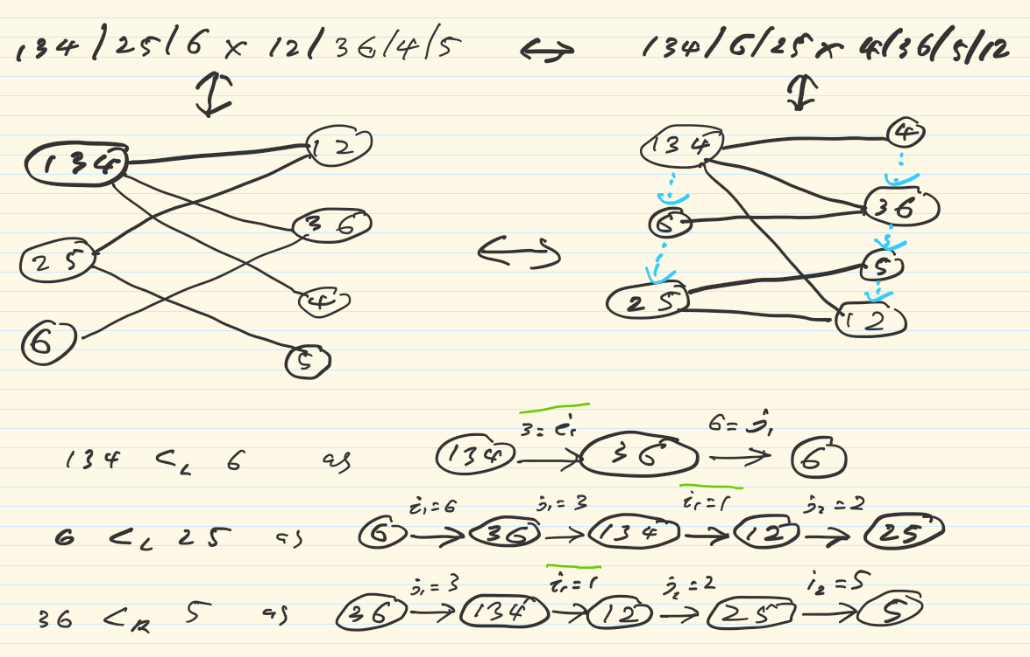
\includegraphics{Images/bijections_example.png}
\end{center}
\caption{The bijection between ordered partitions and bipartite trees.}
\end{figure}

\begin{corollary}[\cite{kajitani1982number}]
The number of essential complementary partitions is $|\EC_n| = 2(n+1)^{n-2}$.
\end{corollary}

\subsection{Bijection with the facets of the diagonal}

In this section we denote by $\OP$ be the set of pairs of ordered partitions of $[n]$ labeling \emph{facets} of the diagonal $\triangle$.

\begin{thm}
\label{thm:facets}
Facets of the diagonal and essential complimentary partitions are in bijection through the inverse functions $u:\OP \to \EC$ and $o:\EC\to \OP$, where
\begin{enumerate}
    \item The function $u$ forgets the order of the ordered partition pair.
    \item The function $o$ uniquely orders an essential complimentary partition pair via the minimal $(I,J)$-pairs defining the diagonal. 
\end{enumerate}
\end{thm}
We shall prove this theorem by establishing the necessary total order, showing that the functions are well defined, and then showing that they are injective.

\begin{lemma} 
\label{u well defined}
The function $u:\OP \to \EC$ that forgets the order in a pair of partitions is well defined.
\end{lemma}
\begin{proof}
Let $P \in \OP_n$. Then $G(u(P))$ is a graph with $l+r=n+1$ vertices, and $n$ edges. Furthermore, as no vertices can be isolated it must be the case that this graph is a tree. 
It is straightforward to verify that $G(u(P))$ must be labeled bipartite tree, but here is how we may explicitly produce the necessary distinct representatives using an algorithm of \cite[Theorem 2]{kajitani1982number}.

Let $G'$ be a copy of $G(u(P))$. 
While there is a vertex of degree $1$ in $G'$ delete it and add the sole edge of that vertex as a distinct representative of the corresponding partition of that vertex. 
As $G'$ is a tree this process can continue until there is a single edge connecting two vertices of degree $1$. 
This edge specifies the element $p$ of the distinct representatives.
\end{proof}

\begin{construction} 
\label{Order Lemma}
For $P=(P_L,P_R) \in \EC$ an essential complementary pair, we construct total orders on $P_L$ and $P_R$ in three steps:
\begin{enumerate}
    \item For $l,l' \in L$ there exists a unique minimal set of edges $p_{l,l'}$ of even cardinality connecting $V(P_l)$ and $V(P_{l'})$ in $G(P)$ (similar for $R$). We partition this set of edges as $I\cup J$ where $I$ and $J$ are each pairwise non-adjacent, and $I$ contains the minimal edge.
    \item Orient each path so that $I$ points left to right, and $J$ points right to left (same orientation for $P_L$ and $P_R$). 
    \item We say $P_l< P_{l'}$ (or $P_r < P_{r'}$) if the constructed path points from $V(P_l) \to V(P_{l'})$ ($V(P_r) \to V(P_{r'})$.
\end{enumerate}
\end{construction}

\begin{proof}
We first show our binary relation is well defined before verifying that it defines a total order on $G(P)$ and hence $P$ via the bijection of \cref{EC Graph Bijection}.

As $G(P)$ is a bipartite tree, every vertex is connected, and every path connecting two vertices on the same side must be of even length. 
As $I$ and $J$ are each pairwise non-adjacent, they must partition the path in an alternating fashion i.e. $p=(I_{i_1},J_{j_1},I_{i_2},J_{j_2},..., )$, hence we can orient the path by forcing $I$ to point left and $J$ to point right.

This order is clearly total, reflexive (by convention) and anti-symmetric, what remains to be checked is its transitivity. 

Let $p_{ab}$ denote the unique maximal path between two vertices $a$ and $b$ on the left of $G(P)$, that is two blocks of $P_L$. 
Let $I_{ab}$ denote the set of left-to-right edges in this path, and let $J_{ab}$ denote its complement. 
Then, we have 
\begin{equation}
    \label{eq:order}
    a < b \iff \min(I_{ab}\cup J_{ab})=\min(I_{ab}) \ . 
\end{equation}
Suppose now that $a < b$ and $b < c$.
Since $p_{ac}= (p_{ab} \cup p_{bc}) \setminus (p_{ab} \cap p_{bc})$, we have $$ I_{ac}=(I_{ab}\cup I_{bc}) \setminus (J_{ab} \cup J_{bc}) \text{ and } J_{ac}=(J_{ab}\cup J_{bc}) \setminus (I_{ab} \cup I_{bc}) \ , $$ and from the condition (\ref{eq:order}) above it is clear that $\min(I_{ac}\cup J_{ac})=\min(I_{ac})$, which completes the proof of the transitivity for the total order on $P_L$. 
The proof for $P_R$ is similar. 
\end{proof}

This order far from being arbitrary provides the unique way to order an essential complimentary partition pair into an ordered partition pair of $\triangle$, as we shall demonstrate next.

First we need a geometrical lemma. 
\begin{proposition}
    The paths between adjacents vertices of $P_L$ or $P_R$ are in bijection with the minimal $(I,J)$-pairs.
\end{proposition}

\begin{proof}
    By \cref{p:minimal-IJ-pairs}, it suffices to show that the paths between adjacent vertices of $P_L$ are in bijection with the solutions of the system of equations of the form $(\rho^1,\sigma^2)$. 
    To ease notation let us write $\rho$ for $\rho^1$ and $\sigma$ for $\sigma^1$. 
    Suppose that $\rho$ is obtained from $\sigma$ by merging the two blocks $\sigma_a$ and $\sigma_b$. 
    The two equations $\langle \vec \sigma_a, x \rangle =0$ and $\langle \vec \sigma_b, x \rangle =0$ now become $\langle \vec \sigma_a + \vec \sigma_b, x \rangle =0$; nothing else changes in the system. 
    Since the solution to the system $(\sigma^1,\sigma^2)$ was $x=0$, now the solution is of dimension $1$, and it is given precisely by the path between $a$ and $b$ in $G(P)$.
    Such a path is given by an alternating sequence of vertices and edges $\sigma_1:=\sigma_a, e_1, \sigma_2, e_2, \ldots, e_{k-1}, \sigma_k:=\sigma_b$. 
    Every edge $e_i \in \{1,\ldots, n\}$ is by definition the intersection $\sigma_{i} \cap \sigma_{i+1}$; thus it is the only common non-zero coordinate between $\vec \sigma_{i}$ and $\vec \sigma_{i+1}$.
    Thus the path encodes the series of equations $x_{e_1}+x_{e_{k-1}}=0$, $x_{e_1}+x_{e_2}=0$, $x_{e_2}+x_{e_3}=0$, $\ldots$, $x_{e_{k-2}}+x_{e_{k-1}}=0$. 
    Thus, $x_{e_1}=1$, $x_{e_2}=-1$, $x_{e_3}=1$, $\ldots$, $x_{e_{k-2}}=1$, $x_{e_{k-1}}=-1$ is a basis of one-dimensional space of solutions, and it gives the corresponding minimal $(I,J)$-pair. 
\end{proof}

\begin{lemma} 
\label{o well defined}
The function $o:\EC \to \OP$ that orders an essential complimentary pair is well defined.
\end{lemma}

\begin{proof}
Let $P=(P_L,P_R) \in \EC$ and consider $o(P)$. 
We first show that every $(I,J)$-condition, for $(I,J) \in D(n)$, which corresponds to a path between vertices is satisfied. 
In particular, this statement will be true for minimal $(I,J)$-pairs, which will be enough in virtue of \cref{p:minimal}. 
Suppose $I,J$ corresponds to a path between two vertices on the left, i.e.
\begin{align*}
    V(P_l) = V_{L_1} \xrightarrow{i_1} V_{R_1}\xrightarrow{j_1} V_{L_2} \xrightarrow{i_2}... \xrightarrow{i_{k}} V_{R_{k-1}} \xrightarrow{j_k} V_{L_k}=V(P_{l'})
\end{align*}
By construction we have that $I = \{i_1,...,i_k\},J=\{j_1,...,j_k\} \in D(n)$ (note we are ordering $I$ and $J$ by the path, so it is not necessarily the case that $\min I = i_1$). 
Furthermore, each sub partition of $P_R$ either contains a single element of $I$ and a single element of $J$, or it contains no elements of $I$ and no elements of $J$. 
As such for any ordering of the sub-partitions of $P_R$ we have that 
\begin{align*}
    \forall m, \bigg|\bigcup_{1\leq k \leq m} P_{R,k} \cap I \bigg| = \bigg|\bigcup_{1\leq k \leq m} P_{R,k} \cap J \bigg|
\end{align*}
Hence in order for this $D(n)$ condition to be satisfied it must be the case that for some ordering of the sub-partitions of $P_L$ we have
\begin{align*}
    \exists m, \bigg| \bigcup_{1\leq k \leq m} P_{L,k} \cap I \bigg| > \bigg|\bigcup_{1\leq k \leq m} P_{L,k} \cap J \bigg|
\end{align*}
Every sub-partition of $P_L$ excluding the $l$th and $l'$th either contains no elements of both $I$ and $J$, or it contains a single element of $I$ and a single element of $J$. 
So the only way for the condition to be satisfied is for $P_l$ to come before $P_{l'}$, which is precisely what is required by the total order.

If $I,J$ correspond to a path between two vertices on the right,
\begin{align*}
    V(P_r) = V_{R_1} \xrightarrow{j_1} V_{L_1}\xrightarrow{i_1} V_{L_2} \xrightarrow{j_2}... \xrightarrow{j_{k}} V_{L_{k-1}} \xrightarrow{1_k} V_{R_k}=V(P_{r'})
\end{align*}
then a similar chain of logic implies we must have an ordering of the sub-partitions of $P_R$ such that
\begin{align*}
    \exists m, |\bigcup_{1\leq k \leq m} P_{R,k} \cap I| < |\bigcup_{1\leq k \leq m} P_{R,k} \cap J|
\end{align*}
and this can only happen if $P_r$ comes before $P_{r'}$.
\end{proof}

\begin{rem}
    It would be interesting to know if there is a geometrical interpretation of the paths that are not between adjacent vertices. 
\end{rem}

To complete the proof of \cref{thm:facets}, it remains to show that both $u:\OP \to \EC$ and $o:\EC\to \OP$ are injective, with the other function being their inverse.

\begin{proof}[{Proof of \cref{thm:facets}}]
The forgetful function $u$ is clearly the inverse to $o$ as forgetting any assigned order will clearly return the original essential complimentary partition pair. 
The ordering function $o$ is the inverse to $u$ as it returns the sole ordering of the sub-partitions which is compatible with the $D(n)$ conditions.
\end{proof}



